\section*{11/10}
	
		\begin{center}
		\textbf{Двумерные краевые задачи}
	\end{center}
	\begin{equation} \label{2d_eq}
	-\frac{\partial}{\partial x} \left( K \frac{\partial u}{\partial x} \right) -\frac{\partial}{\partial y} \left( K \frac{\partial u}{\partial y} \right) + bu = f
	\end{equation}
	
	$K(x, y),\ b(x, y),\ f(x,y)$ -- заданные (гладкие) функции.
	
	$u(x, y)$ -- неизвестная.
	
	$\Omega$ -- область, где задано уравнение \eqref{2d_eq}, $\Gamma$ -- граница $\Omega$ .
	\\
	
	\begin{center}
	\begin{tikzpicture}
    % Ось координат
    \draw[->] (-1,0) -- (5,0);
    \draw[->] (0,-1) -- (0,5);
    
    % Кардиоида
        \draw[domain=0:360,samples=200,smooth,variable=\t,rotate=-90,scale=0.5,shift={(3,3)}]
        plot ({2*(1-cos(\t)) * cos(\t) - 6}, {2*(1-cos(\t)) * sin(\t) + 2});
        
        \draw[->,color=red,domain=270:340,samples=200,smooth,variable=\t,rotate=-90,scale=0.5,shift={(3,3)}]
        plot ({2*(1-cos(\t)) * cos(\t) - 6}, {2*(1-cos(\t)) * sin(\t) + 2}) node[below] {$\xi$};
        
        \draw[thick,color=blue,domain=200:240,samples=200,smooth,variable=\t,rotate=-90,scale=0.5,shift={(3,3)}]
        plot ({2*(1-cos(\t)) * cos(\t) - 6}, {2*(1-cos(\t)) * sin(\t) + 2}) node[above left] {$\Gamma_1$};
        
        \draw[->] (3, 1.25) -- (3, 0.5) node[right] {$\vec n$};
        
        \node at (3, 2) {$\Omega$};
        \node at (4, 1.5) {$\Gamma_2$};
        
\end{tikzpicture}
\end{center}
	
	Замкнутый контур $\Gamma$ -- гладкий, за исключением конечного числа угловых точек, в которых внутренний угол $\alpha \in [0; \pi]$.
	\[\Gamma = \underbrace{\Gamma_1}_{\text{I рода}} \cup \underbrace{\Gamma_2}_{\text{II/III рода}}\]
	\begin{center}
		$u(\xi) = \hat u(\xi)$ -- на $\Gamma_1$ (заданное значение).
	\end{center}
	\[K(\xi)\frac{\partial u}{\partial n} = \hat \sigma (\xi) - \text{ на } \Gamma_2\]
	\[\frac{\partial u}{\partial n} = \frac{\partial u}{\partial x} l_x + \frac{\partial u}{\partial y} l_y,\ 
	\begin{cases}
	l_x = \cos(\alpha x) = \cos(\vec x, \vec n),\\
	l_y = \cos(\alpha y) = \cos(\vec y, \vec n),\\
	||\vec n|| = 1
	\end{cases}\]

\begin{center}
	\begin{tikzpicture}
	\draw[thick] (0,0) arc[start angle=0, end angle=90, radius=3cm];

    	% Нормаль к гипотенузе
    	\coordinate (A) at (-0.18,0.93);
   	\coordinate (B) at (-2.5,2.93);
    	\coordinate (C) at (-2.5,0.93);
     	\coordinate (MidAB) at ($ (A)!0.5!(B) $);
	    
    	% Вектор нормали
    	\draw[->, thick, blue] (MidAB)++(0.31,0.31) -- ++(1.5,1.5) node[right] {$\vec n$};
	\draw[->] (MidAB)++(0.31,0.31) -- ++(0, 1.5) node[left] {$l_y$};
	\draw[->] (MidAB)++(0.31,0.31) -- ++(1.5, 0) node[below] {$l_x$};
	\draw[thick] (MidAB)++(0.71, 0.31) arc[start angle=0, end angle=47, radius=0.4cm] node[right] {$\alpha_x$};
	\draw[thick] (MidAB)++(0.31, 0.71) arc[start angle=90, end angle=47, radius=0.4cm] node[above] {$\alpha_y$};
	\draw[dashed] (MidAB)++(0.31,1.81) -- ++(1.5, 0);
	\draw[dashed] (MidAB)++(1.81,0.31) -- ++(0, 1.5);

	\end{tikzpicture}
	\end{center}
	
	Составим невязку:
	\[r(x, y) = -\frac{\partial}{\partial x} \left( K \frac{\partial u}{\partial x} \right) -\frac{\partial}{\partial y} \left( K \frac{\partial u}{\partial y} \right) + bu - f = 0\]
	
	\[\iint\limits_{\Omega} r(x, y) \cdot v \, dx \, dy = 0,\]
	
	где $v(x, y)$ -- пробная (гладкая) функция; на $\Gamma_1$: $v = 0$
	
	\begin{equation}\label{iint}
	\iint\limits_{\Omega} \left [ -\frac{\partial}{\partial x} \left( K \frac{\partial u}{\partial x} \right) -\frac{\partial}{\partial y} \left( K \frac{\partial u}{\partial y} \right) + bu - f \right ] \cdot v \, dx \, dy = 0
	\end{equation}
	
	Рассмотрим первый интеграл:
	\[-\iint\limits_{\Omega} \frac{\partial}{\partial x} \left( K \frac{\partial u}{\partial x} \right) \cdot v \, dx \, dy\]
	
	Формула Гаусса-Остроградского:
	\[\iint\limits_{\Omega} \frac{\partial}{\partial x} F dx dy = \int \limits_{\Gamma} F \cdot l_x d \xi\]
	
	Представим $F$ в виде $F = uv$:
	\[\frac{\partial}{\partial x} F = \frac{\partial}{\partial x} (uv) = \frac{\partial u}{\partial x} v + u \frac{\partial v}{\partial x}\ \Rightarrow\ 
	\frac{\partial u}{\partial x} v = \frac{\partial}{\partial x} (uv) - u \frac{\partial v}{\partial x}\]
	
	Отсюда:
	\[\iint\limits_{\Omega} \frac{\partial u}{\partial x} v \, dx \, dy = \iint\limits_{\Omega} \left( \frac{\partial}{\partial x} (uv) - u \frac{\partial v}{\partial x} \right) \, dx \, dy\]
	
	И по формуле Гаусса-Остроградского:
	\[\iint\limits_{\Omega} \frac{\partial u}{\partial x} v \, dx \, dy = \int \limits_{\Gamma} uv \cdot l_x d \xi - \iint\limits_{\Omega} \frac{\partial v}{\partial x} u \, dx \, dy\]
	
	Тогда:
	\[-\iint\limits_{\Omega} \frac{\partial}{\partial x} \left( K \frac{\partial u}{\partial x} \right) \cdot v \, dx \, dy = 
	-\int \limits_{\Gamma} K \cdot \frac{\partial u}{\partial x} \cdot v \cdot l_x d \xi + \iint\limits_{\Omega} \frac{\partial v}{\partial x} \left(  K \cdot \frac{\partial u}{\partial x} \right) \, dx \, dy\]
	\[-\iint\limits_{\Omega} \frac{\partial}{\partial y} \left( K \frac{\partial u}{\partial y} \right) \cdot v \, dx \, dy = 
	-\int \limits_{\Gamma} K \cdot \frac{\partial u}{\partial y} \cdot v \cdot l_y d \xi + \iint\limits_{\Omega} \frac{\partial v}{\partial y} \left(  K \cdot \frac{\partial u}{\partial y} \right) \, dx \, dy\]
	
	Подставим в \eqref{iint}:
	\[\iint\limits_{\Omega} \left [ \frac{\partial v}{\partial x} \cdot K \cdot \frac{\partial u}{\partial x} + \frac{\partial v}{\partial y} \cdot K \cdot \frac{\partial u}{\partial y} + bu \cdot v - f  \cdot v \right ] \, dx \, dy -\]
	\[-\int \limits_{\Gamma_2} K \cdot v \cdot \left(\frac{\partial u}{\partial x} \cdot l_x + \frac{\partial u}{\partial y} \cdot l_y \right) = 0\]

	\underline{Задача упругости}
 	$ u(x, y) $ - перемещения \\
 	\[ \varepsilon = [\varepsilon_x \quad \varepsilon_y]^T, \quad \varepsilon_x = - \frac{\partial u}{\partial y},\quad \varepsilon_y = - \frac{\partial u}{\partial y} \]
	\[ \varepsilon = Lu,\quad L = \left[- \frac{\partial}{\partial x} \quad - \frac{\partial}{\partial y}\right]^T \]
	\[ \sigma = k \varepsilon = kLu \]
	\begin{center}
	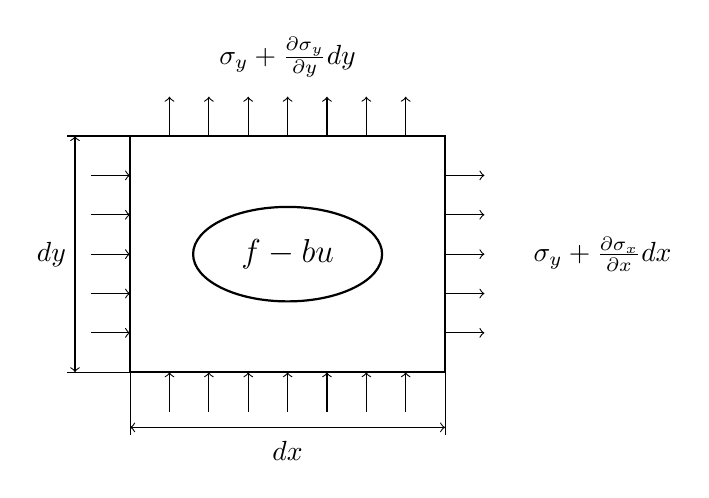
\begin{tikzpicture}
    % Прямоугольник
    \draw[thick] (0, 0) rectangle (4, 3);
    
    % Центральная фигура (овал)
    \draw[thick] (2, 1.5) ellipse (1.2 and 0.6);
    \node at (2, 1.5) {\large $f - bu$};  % Текст внутри овала
    
    % Горизонтальные стрелки (слева направо)
    \foreach \y in {0.5, 1, 1.5, 2, 2.5} {
        \draw[->] (-0.5, \y) -- (0, \y);
    }
    
    % Вертикальные стрелки (снизу вверх)
    \foreach \x in {0.5, 1, 1.5, 2, 2.5, 3, 3.5} {
        \draw[->] (\x, -0.5) -- (\x, 0);
    }

    % Горизонтальные стрелки справа
    \foreach \y in {0.5, 1, 1.5, 2, 2.5} {
        \draw[->] (4, \y) -- (4.5, \y);
    }
    
    % Вертикальные стрелки сверху
    \foreach \x in {0.5, 1, 1.5, 2, 2.5, 3, 3.5} {
        \draw[->] (\x, 3) -- (\x, 3.5);
    }
    
    % Подписи координат
    \draw[thin] (0, 0) -- (0, -0.8);
    \draw[thin] (4, 0) -- (4, -0.8);
    \draw[<->][thin] (0, -0.7) -- (4, -0.7);
    \node at (2, -1) {$dx$};    % Горизонтальная разметка снизу
    
    \draw[thin] (0, 0) -- (-0.8, 0);
    \draw[thin] (0, 3) -- (-0.8, 3);
    \draw[<->][thin] (-0.7, 0) -- (-0.7, 3);
    \node at (-1, 1.5) {$dy$};  % Вертикальная разметка слева
    
    \node at (2, 4) {$\sigma_y + \frac{\partial \sigma_y}{\partial y} dy$};
    \node at (6, 1.5) {$\sigma_y + \frac{\partial \sigma_x}{\partial x} dx$};

    % Дополнительные стрелки от центрального овала
    %\foreach \angle in {-40, -20, 0, 20, 40} {
        %\draw[->] (2, 1.5) -- ++(\angle:1.5);
   % }

\end{tikzpicture}
\end{center}
	\[ d \Omega = dxdy \]
	\[ \sigma_x dy + \sigma_y dx + (f-bu) dxdy = \left(\sigma_x + \frac{\partial \sigma_x}{\partial x}dx\right) dy + \left(\sigma_y + \frac{\partial \sigma_y}{\partial y}dy\right) dx \]
	\[ \frac{\partial \sigma_x}{\partial x} + \frac{\partial \sigma_y}{\partial y} = f - bu \]
	\[ L_* = \left[\frac{\partial}{\partial x} \quad \frac{\partial}{\partial y}\right],\quad L_* = -L^T,\ \  L_* \sigma = L_*kLu = f - bu \]
	\[ \left[\frac{\partial}{\partial x} \quad \frac{\partial}{\partial y}\right] \cdot k \cdot 
	\begin{bmatrix}
		-\frac{\partial u}{\partial x}\\
		- \frac{\partial u}{\partial y}
	\end{bmatrix}
 	= f-bu \]
	\[-\frac{\partial}{\partial x} \left ( K \frac{\partial u}{\partial x} \right) - \frac{\partial}{\partial y} \left ( K \frac{\partial u}{\partial y} \right) = f \cdot bu \Leftrightarrow \eqref{2d_eq}\]
	
	\begin{center}
	\begin{tikzpicture}
	\draw[thick] (0,0) arc[start angle=0, end angle=90, radius=3cm] node[left] {$\Gamma_2$};
	\foreach \angle in {10, 20, 30, 40, 50, 60, 70, 80} {
        % Координаты точек на окружности
        \coordinate (P) at ({3*cos(\angle) - 3}, {3*sin(\angle)});
        % Координаты направления нормали
        \coordinate (N) at ({0.5*cos(\angle)}, {0.5*sin(\angle)});
        % Рисуем нормали
        \draw[<-] (P) -- ++(N);
    }

	\draw[thick] (-0.18,0.93) -- (-2.5,2.93) -- (-2.5,0.93) -- cycle;
	\node at (-1.5, 1.15) {\footnotesize$dx$};
	\node at (-2.25, 1.93) {\footnotesize$dy$};

    	% Нормаль к гипотенузе
    	\coordinate (A) at (-0.18,0.93);
   	\coordinate (B) at (-2.5,2.93);
    	\coordinate (C) at (-2.5,0.93);
     	\coordinate (MidAB) at ($ (A)!0.5!(B) $);
	
	\node[left] at (MidAB) {\footnotesize$d\xi$};
    
    	% Вектор нормали
    	\draw[->, thick, blue] (MidAB) -- ++(1,1.15) node[right] {$\vec n$};
	\draw[dashed] (MidAB) -- ++(0, 1.5);
	\draw[dashed] (MidAB) -- ++(1.5, 0);
	\draw[thick] (MidAB)++(0.4, 0) arc[start angle=0, end angle=47, radius=0.4cm] node[right] {$\alpha_x$};
	\draw[thick] (MidAB)++(0, 0.4) arc[start angle=90, end angle=47, radius=0.4cm] node[above] {$\alpha_y$};
	
	\draw[->] (-3,0.93) -- (-2.5,0.93);
	\draw[->] (-3,1.33) -- (-2.5,1.33);
	\draw[->] (-3,1.73) -- (-2.5,1.73);
	\draw[->] (-3,2.13) -- (-2.5,2.13);
	\draw[->] (-3,2.53) -- (-2.5,2.53);
	\draw[->] (-3,2.93) -- (-2.5,2.93);
	
	\draw[->] (-2.4,0.43) -- (-2.4,0.93);
	\draw[->] (-2,0.43) -- (-2,0.93);
	\draw[->] (-1.6,0.43) -- (-1.6,0.93);
	\draw[->] (-1.2,0.43) -- (-1.2,0.93);
	\draw[->] (-0.8,0.43) -- (-0.8,0.93);
	\draw[->] (-0.4,0.43) -- (-0.4,0.93);
	
	\node at (-3, 0.5) {$\Omega$};
	\end{tikzpicture}
	\end{center}
	\[\Gamma_1: u(\xi) = \hat u(\xi)\]
	\[dx = \cos \alpha_y d\xi = l_y d\xi,\ \ dy = \cos \alpha_x d\xi = l_x d\xi\]
	\[\sigma_y dx + \sigma_x dy + \hat \sigma d\xi = 0,\ \ \sigma_x = K \varepsilon_x = -K \frac{\partial u}{\partial x},\ \sigma_y = K \varepsilon_y = -K \frac{\partial u}{\partial y}\]
	
	Тогда:
	\[-K \frac{\partial u}{\partial y} dx -K \frac{\partial u}{\partial x} dy + \hat \sigma d\xi = 0,\ \ -K \frac{\partial u}{\partial y} l_y d\xi -K \frac{\partial u}{\partial x} l_x d\xi + \hat \sigma d\xi = 0\]
	\[K \frac{\partial u}{\partial n} = \hat \sigma\]
	
	Отсюда:
	\begin{equation}\label{2d_eq_2}
	\iint \limits_{\Omega} \left(\frac{\partial v}{\partial x} K \frac{\partial u}{\partial x} + \frac{\partial v}{\partial y} K \frac{\partial u}{\partial y} + bu \cdot v - f \cdot v\right) dx dy - \\
	\int \limits_{\Gamma} \underbrace{ \left(K \frac{\partial u}{\partial x} l_x + K \frac{\partial u}{\partial y} l_y\right)}_{K \cdot \frac{\partial u}{\partial n} = \hat \sigma(\xi)}  \cdot v d\xi = 0 
	\end{equation}
	
	\[\iint \limits_{\Omega} ((Lu)^T K (Lu) + v^T bu - v^T f) dxdy - \int \limits_{\Gamma_2} v^T \hat \sigma d\xi = 0\]